\documentclass[12pt,a4paper,twoside]{article}

% Packages
\usepackage[margin=1in]{geometry}
\usepackage{cite}
\usepackage{amsmath,amssymb,amsfonts}
\usepackage{graphicx}
\usepackage{textcomp}
\usepackage{xcolor}
\usepackage[hidelinks]{hyperref}
\usepackage{listings}
\usepackage{titlesec}
\usepackage{tikz}
\usepackage{booktabs}
\usepackage{float}
\usepackage{fancyhdr}
\usepackage[font=small,labelfont=bf]{caption}
\usetikzlibrary{shapes.geometric, arrows.meta, positioning, calc, fit}

% Graphics path - figures are stored in results/figures
\graphicspath{{../results/figures/}}

% Header/footer setup
\pagestyle{fancy}
\fancyhf{}
\fancyhead[LE]{Reinforcement Learning Applied to the Snake Game}
\fancyhead[RO]{Al-Amri, Al-Ubejdij, Al-Moslemani, Humaid, Aldous, Gavankar}
\fancyfoot[C]{\thepage}
\renewcommand{\headrulewidth}{0.4pt}

% No paragraph indentation
\setlength{\parindent}{0pt}
\setlength{\parskip}{6pt}

% Document metadata
\def\BibTeX{{\rm B\kern-.05em{\sc i\kern-.025em b}\kern-.08em
    T\kern-.1667em\lower.7ex\hbox{E}\kern-.125emX}}

\begin{document}

\title{Reinforcement Learning Applied to the Snake Game\\
\large ECEN 446 Course Project\\[1em]
\normalsize Instructor: Dr. Joseph Boutros}

\author{
Elyas Al-Amri \and
Ejmen Al-Ubejdij \and
Ahmad Al-Moslemani \and
Marwan Humaid \and
Hamad Aldous \and
Umair Gavankar
}

\date{\today}

\maketitle

% Table of contents on separate page
\newpage
\setcounter{tocdepth}{2}
\tableofcontents
\newpage

%==============================================================================
% ABSTRACT
%==============================================================================
\begin{abstract}
This report presents a comprehensive investigation of reinforcement learning techniques applied to the classic Snake game. We implement and evaluate multiple algorithms including Deep Q-Networks (DQN) with various enhancements (Double DQN, Dueling DQN, Prioritized Experience Replay, and Noisy Networks), as well as policy gradient methods (REINFORCE, Advantage Actor-Critic, and Proximal Policy Optimization). Our work extends beyond single-agent scenarios to include competitive two-snake environments with curriculum learning. We design and compare multiple state representations, from basic 11-dimensional feature vectors to enhanced 24-dimensional representations incorporating flood-fill reachability metrics. Experimental results demonstrate that PPO with flood-fill features achieves superior performance in single-snake scenarios, while curriculum learning proves essential for training competitive agents in two-snake environments. The flood-fill feature, which measures reachable free space, emerges as a critical component for avoiding self-trapping behaviors. We also implement GPU-accelerated vectorized environments achieving 100-300x speedup over sequential training. This work provides practical insights into algorithm selection, state representation design, and training strategies for game-playing agents.
\end{abstract}

%==============================================================================
% SECTION 1: INTRODUCTION
%==============================================================================
\section{Introduction}

Reinforcement Learning (RL) has emerged as one of the most powerful paradigms in artificial intelligence, enabling agents to learn optimal behaviors through interaction with their environment \cite{sutton2018reinforcement}. Unlike supervised learning, where labeled examples guide the learning process, RL agents learn from the consequences of their actions through rewards. This fundamental characteristic makes RL especially suitable for sequential decision-making problems, including game playing, robotics, and autonomous systems.

The success of RL in recent years has been remarkable. DeepMind's breakthrough with Deep Q-Networks (DQN) demonstrated that deep neural networks could learn to play Atari games directly from raw pixel inputs, achieving human-level performance across multiple games \cite{mnih2015human}. This achievement marked a pivotal moment in AI research, showing that the combination of deep learning and reinforcement learning could tackle problems previously thought to require extensive hand-crafted features and domain knowledge. Subsequent advances, including AlphaGo's victory over world champion Go players \cite{silver2016mastering} and the application of RL to complex robotic control tasks, have further demonstrated the potential of these methods.

\subsection{Problem Statement}

This project develops and evaluates reinforcement learning agents capable of playing the Snake game effectively. Our objectives encompass implementing both single-snake and two-snake competitive environments that adhere to the standard Gymnasium (OpenAI Gym) interface, providing a consistent API for RL algorithm interaction. We design multiple state representations that capture relevant spatial and strategic information while remaining tractable for learning algorithms, ranging from basic feature vectors to enhanced representations with flood-fill reachability metrics.

We implement and compare multiple RL algorithms spanning value-based methods (DQN and its variants) and policy gradient methods (REINFORCE, A2C, PPO). For competitive scenarios, we develop curriculum learning approaches that progressively increase opponent difficulty from static to co-evolving agents. Finally, we evaluate performance through metrics such as average score, survival rate, and win rate in competitive settings, analyzing the learned behaviors and providing practical recommendations for algorithm selection.

\subsection{Motivation}

The Snake game, while simple in its rules, presents several interesting challenges for reinforcement learning. The game requires the agent to navigate a bounded grid environment, collect food items to maximize score, avoid collisions with walls and its own growing body, plan ahead to avoid becoming trapped, and balance exploration (finding food) with safety (avoiding death). These challenges make Snake an ideal testbed for RL algorithms.

The game's discrete action space (typically 3 or 4 directions) and deterministic dynamics simplify the learning problem compared to continuous control tasks, yet the increasing difficulty as the snake grows longer and the sparse reward structure (only receiving reward when eating food or dying) present meaningful learning challenges. Furthermore, the Snake game serves as an excellent educational platform for understanding core RL concepts. The game's simplicity allows us to focus on fundamental RL principles without being overwhelmed by environmental complexity, while still requiring sophisticated learning strategies to achieve high performance.

We also want to experiment with RL in different settings: when an agent learns with or against another agent. We created a two-snake variant where both snakes compete for food on a shared grid. This competitive variant introduces additional challenges including opponent modeling, strategic planning, and handling non-stationarity in the environment. Multi-agent reinforcement learning (MARL) in competitive settings has gained significant attention due to its applications in game AI, autonomous driving, and economic modeling \cite{lowe2017multi}.

\subsection{Measure for Success and Understanding}

We define success for this project along two dimensions: generalization and adaptability to different settings.

\textbf{Grid Size Adaptability.} A well-designed RL agent should not be restricted to a single grid size. By using a feature-based state representation rather than raw grid pixels, our agents can generalize to arbitrary grid dimensions without retraining. The feature encoder extracts relative spatial information (danger indicators, food direction, flood-fill ratios) that remains meaningful regardless of absolute grid size. We demonstrate this by training on a $10 \times 10$ grid and evaluating on larger grids.

\textbf{Applying RL in Different Settings.} Beyond single-agent performance, we extend our investigation to competitive multi-agent scenarios. The two-snake environment tests whether RL techniques can handle non-stationary opponents, strategic decision-making under competition, and the credit assignment problem when outcomes depend on multiple agents' actions. Success in this setting requires curriculum learning and careful reward design, demonstrating the broader applicability of RL beyond simple single-agent tasks.

The remainder of this report is organized as follows. Section 2 provides theoretical background on reinforcement learning, covering Markov Decision Processes, value functions, and both value-based and policy-based learning methods. Section 3 details our implementation including code structure, GPU vectorization, and state representations. Section 4 presents experimental results for single-snake and two-snake scenarios. Section 5 discusses findings and insights. Finally, Section 6 concludes with limitations and future directions.

%==============================================================================
% SECTION 2: BACKGROUND AND THEORY
%==============================================================================
\section{Background and Theory}

Reinforcement learning provides a mathematical framework for learning optimal behavior through trial and error. Unlike supervised learning, where correct actions are explicitly provided, RL agents must discover which actions yield the most reward by interacting with their environment. This section presents the theoretical foundations underlying modern RL algorithms, beginning with the formal framework of Markov Decision Processes and progressing through value-based and policy-based learning methods.

\subsection{Markov Decision Processes}

A Markov Decision Process (MDP) provides the mathematical foundation for formulating reinforcement learning problems \cite{sutton2018reinforcement}. An MDP is defined by a tuple $(\mathcal{S}, \mathcal{A}, P, R, \gamma)$ where $\mathcal{S}$ is the state space representing all possible states the environment can be in, $\mathcal{A}$ is the action space representing all possible actions the agent can take, $P: \mathcal{S} \times \mathcal{A} \times \mathcal{S} \rightarrow [0,1]$ is the state transition probability function where $P(s'|s,a)$ denotes the probability of transitioning to state $s'$ when taking action $a$ in state $s$, $R: \mathcal{S} \times \mathcal{A} \rightarrow \mathbb{R}$ is the reward function where $R(s,a)$ gives the immediate reward for taking action $a$ in state $s$, and $\gamma \in [0,1]$ is the discount factor determining the present value of future rewards.

The fundamental assumption of an MDP is the Markov property: the future state depends only on the current state and action, not on the history of past states and actions. Formally:
\begin{equation}
P(s_{t+1}|s_t, a_t, s_{t-1}, a_{t-1}, \ldots, s_0, a_0) = P(s_{t+1}|s_t, a_t)
\end{equation}

This memoryless property significantly simplifies the decision-making process, as the agent only needs to consider the current state rather than maintaining the complete history.

The goal of reinforcement learning is to find an optimal policy $\pi^*$ that maximizes the expected cumulative discounted reward, also called the \textbf{return}:
\begin{equation}
G_t = \sum_{k=0}^{\infty} \gamma^k R_{t+k+1}
\end{equation}
where $R_{t+k+1}$ is the reward received at time step $t+k+1$. The discount factor $\gamma$ serves two purposes: it ensures that the infinite sum converges (when $\gamma < 1$), and it expresses the preference for immediate rewards over delayed rewards.

\begin{figure}[H]
\centering
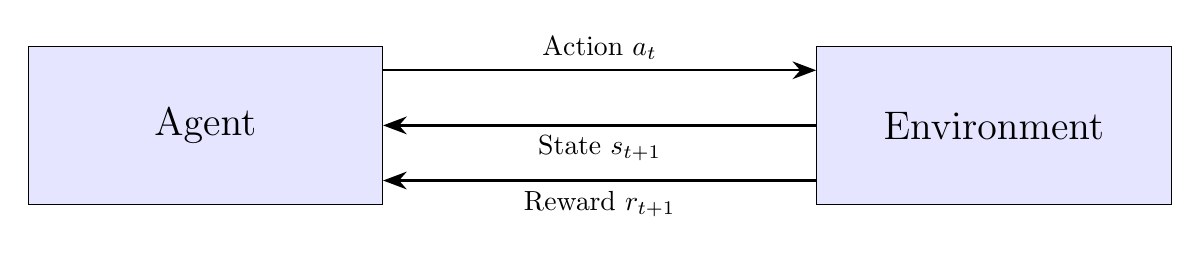
\begin{tikzpicture}[
    node distance=2.5cm,
    block/.style={rectangle, draw, minimum width=4.5cm, minimum height=2cm, align=center, fill=blue!10, font=\Large},
    arrow/.style={-{Stealth[length=3mm]}, thick}
]
    % Agent
    \node[block] (agent) {Agent};

    % Environment
    \node[block, right=5.5cm of agent] (env) {Environment};

    % Arrows - well spaced
    \draw[arrow] ([yshift=0.7cm]agent.east) -- node[above] {Action $a_t$} ([yshift=0.7cm]env.west);
    \draw[arrow] ([yshift=0cm]env.west) -- node[below] {State $s_{t+1}$} ([yshift=0cm]agent.east);
    \draw[arrow] ([yshift=-0.7cm]env.west) -- node[below] {Reward $r_{t+1}$} ([yshift=-0.7cm]agent.east);

\end{tikzpicture}
\caption{Agent-environment interaction in a Markov Decision Process.}
\label{fig:mdp}
\end{figure}

\subsection{Policy Function}

A \textbf{policy} $\pi$ defines the agent's behavior by specifying which action to take in each state. Policies can be deterministic or stochastic:

\textbf{Deterministic policy:} $\pi: \mathcal{S} \rightarrow \mathcal{A}$ maps states directly to actions. Given state $s$, the agent always takes action $a = \pi(s)$.

\textbf{Stochastic policy:} $\pi(a|s)$ represents the probability of selecting action $a$ when in state $s$. The agent samples actions according to this distribution, enabling exploration of different behaviors.

The choice between deterministic and stochastic policies has important implications. Stochastic policies are essential during learning to ensure exploration of the action space. They also arise naturally in multi-agent settings where predictable behavior can be exploited by opponents. However, for many single-agent tasks, the optimal policy is deterministic.

\subsection{Value Function (State-Value)}

The \textbf{state-value function} $V^\pi(s)$ estimates how good it is for an agent to be in a given state. It gives the expected return when starting in state $s$ and following policy $\pi$ thereafter:
\begin{equation}
V^\pi(s) = \mathbb{E}_\pi[G_t | s_t = s] = \mathbb{E}_\pi\left[\sum_{k=0}^{\infty} \gamma^k R_{t+k+1} \middle| s_t = s\right]
\end{equation}

The state-value function satisfies the \textbf{Bellman equation}:
\begin{equation}
V^\pi(s) = \sum_{a \in \mathcal{A}} \pi(a|s) \sum_{s' \in \mathcal{S}} P(s'|s,a)[R(s,a) + \gamma V^\pi(s')]
\end{equation}

The optimal state-value function is defined as the maximum value achievable over all policies:
\begin{equation}
V^*(s) = \max_\pi V^\pi(s)
\end{equation}

\subsection{Action-Value Function (Q-Function)}

The \textbf{action-value function} (or Q-function) $Q^\pi(s,a)$ estimates how good it is to take a particular action in a given state. It gives the expected return when starting in state $s$, taking action $a$, and following policy $\pi$ thereafter:
\begin{equation}
Q^\pi(s,a) = \mathbb{E}_\pi[G_t | s_t = s, a_t = a]
\end{equation}

The Q-function is particularly useful because it allows action selection without knowing the environment dynamics. Once we have the optimal Q-function $Q^*$, we can extract the optimal policy through:
\begin{equation}
\pi^*(s) = \arg\max_{a \in \mathcal{A}} Q^*(s,a)
\end{equation}

The optimal Q-function satisfies the \textbf{Bellman optimality equation}:
\begin{equation}
Q^*(s,a) = \sum_{s' \in \mathcal{S}} P(s'|s,a)\left[R(s,a) + \gamma \max_{a' \in \mathcal{A}} Q^*(s',a')\right]
\end{equation}

This greedy policy with respect to $Q^*$ is guaranteed to be optimal.

\subsection{On-Policy vs Off-Policy Learning}

A fundamental distinction in reinforcement learning is between on-policy and off-policy methods:

\textbf{On-policy methods} learn the value of the policy being used to make decisions. The agent collects experience using its current policy and updates that same policy based on those experiences. Examples include SARSA, A2C, and PPO. On-policy methods are generally more stable but less sample-efficient, as each experience can only be used once before the policy changes.

\textbf{Off-policy methods} learn the value of a different policy than the one being used to collect data. The agent follows a behavior policy (often exploratory) while learning about a target policy (often greedy). Examples include Q-learning and DQN. Off-policy methods can reuse past experiences through replay buffers, improving sample efficiency, but they can be less stable due to the distribution mismatch between behavior and target policies.

For our Snake game experiments, we employ both paradigms: DQN (off-policy) uses experience replay to learn from stored transitions, while PPO (on-policy) learns directly from freshly collected rollouts.

\subsection{Experience Replay}

Experience replay is a critical technique that enables stable training in deep reinforcement learning. The key insight is that training a neural network on consecutive samples from an agent's trajectory creates two problems: (1) consecutive samples are highly correlated, violating the i.i.d. assumption of stochastic gradient descent, and (2) the data distribution shifts as the policy improves, causing catastrophic forgetting of previously learned behaviors.

\textbf{The Problem Without Replay.} When training directly on sequential experiences, the network sees a stream of highly correlated transitions. For example, in Snake, consecutive states differ only slightly as the snake moves one cell. This correlation causes the gradient updates to be biased toward recent experiences, leading to oscillating or diverging Q-values. The network effectively ``forgets'' how to handle states it encountered earlier in training.

\begin{figure}[H]
\centering
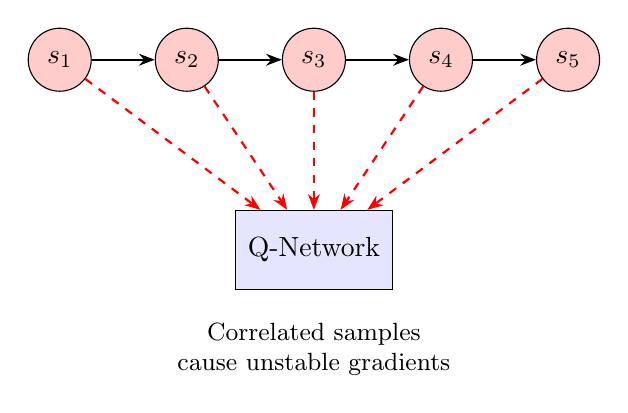
\begin{tikzpicture}[
    node distance=0.8cm,
    state/.style={circle, draw, minimum size=0.8cm, fill=red!20},
    arrow/.style={-{Stealth[length=2mm]}, thick},
    dashedarrow/.style={-{Stealth[length=2mm]}, thick, dashed}
]
    % Sequential states
    \node[state] (s1) {$s_1$};
    \node[state, right=of s1] (s2) {$s_2$};
    \node[state, right=of s2] (s3) {$s_3$};
    \node[state, right=of s3] (s4) {$s_4$};
    \node[state, right=of s4] (s5) {$s_5$};

    \draw[arrow] (s1) -- (s2);
    \draw[arrow] (s2) -- (s3);
    \draw[arrow] (s3) -- (s4);
    \draw[arrow] (s4) -- (s5);

    % Neural network
    \node[rectangle, draw, fill=blue!10, minimum width=2cm, minimum height=1cm, below=1.5cm of s3] (nn) {Q-Network};

    % Correlation indicator
    \draw[dashedarrow, red] (s1) -- (nn);
    \draw[dashedarrow, red] (s2) -- (nn);
    \draw[dashedarrow, red] (s3) -- (nn);
    \draw[dashedarrow, red] (s4) -- (nn);
    \draw[dashedarrow, red] (s5) -- (nn);

    % Label
    \node[below=0.3cm of nn, text width=6cm, align=center, font=\small] {Correlated samples cause unstable gradients};
\end{tikzpicture}
\caption{Without replay: sequential samples are correlated, causing training instability.}
\label{fig:no_replay}
\end{figure}

\textbf{The Solution With Replay.} Experience replay addresses these issues by storing transitions $(s_t, a_t, r_{t+1}, s_{t+1})$ in a buffer and sampling mini-batches uniformly at random for training. This breaks temporal correlations and provides a more stationary data distribution. The buffer acts as a memory that allows reusing past experiences multiple times, improving sample efficiency.

\begin{figure}[H]
\centering
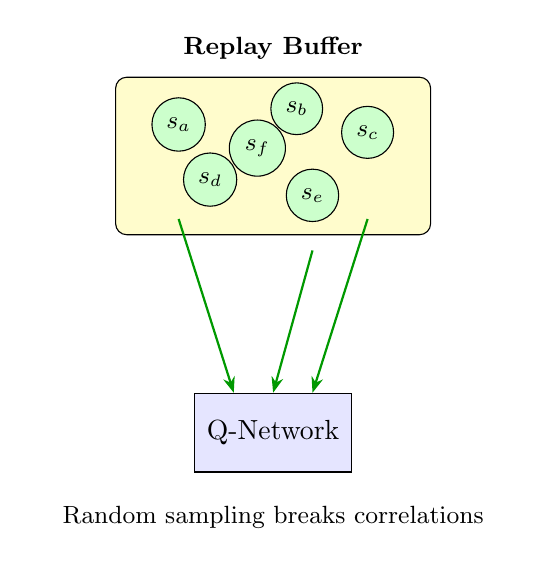
\begin{tikzpicture}[
    node distance=0.6cm,
    state/.style={circle, draw, minimum size=0.6cm, fill=green!20, font=\small},
    arrow/.style={-{Stealth[length=2mm]}, thick},
    dashedarrow/.style={-{Stealth[length=2mm]}, thick, dashed}
]
    % Replay buffer (cylinder-like)
    \node[rectangle, draw, fill=yellow!20, minimum width=4cm, minimum height=2cm, rounded corners] (buffer) {};
    \node[above=0.1cm of buffer.north, font=\small\bfseries] {Replay Buffer};

    % States inside buffer (scattered)
    \node[state] at (-1.2, 0.4) {$s_a$};
    \node[state] at (0.3, 0.6) {$s_b$};
    \node[state] at (1.2, 0.3) {$s_c$};
    \node[state] at (-0.8, -0.3) {$s_d$};
    \node[state] at (0.5, -0.5) {$s_e$};
    \node[state] at (-0.2, 0.1) {$s_f$};

    % Neural network
    \node[rectangle, draw, fill=blue!10, minimum width=2cm, minimum height=1cm, below=2cm of buffer] (nn) {Q-Network};

    % Random sampling arrows
    \draw[arrow, green!60!black] (-1.2, -0.8) -- ([xshift=-0.5cm]nn.north);
    \draw[arrow, green!60!black] (0.5, -1.2) -- (nn.north);
    \draw[arrow, green!60!black] (1.2, -0.8) -- ([xshift=0.5cm]nn.north);

    % Label
    \node[below=0.3cm of nn, text width=6cm, align=center, font=\small] {Random sampling breaks correlations};
\end{tikzpicture}
\caption{With replay: random sampling from buffer decorrelates training data.}
\label{fig:with_replay}
\end{figure}

The replay buffer typically stores the most recent $N$ transitions (e.g., $N = 100,000$), discarding older experiences as new ones arrive. This ensures the buffer contains a diverse set of experiences while remaining bounded in memory.

\subsection{Value-Based Methods}

Value-based methods learn the optimal value function and derive a policy from it. The foundational algorithm in this category is Q-learning \cite{watkins1992q}, which updates Q-values using:
\begin{equation}
Q(s_t, a_t) \leftarrow Q(s_t, a_t) + \alpha \left[R_{t+1} + \gamma \max_{a} Q(s_{t+1}, a) - Q(s_t, a_t)\right]
\end{equation}
where $\alpha$ is the learning rate. The term in brackets is the temporal difference (TD) error, measuring the discrepancy between the current estimate and the bootstrapped target.

For problems with large or continuous state spaces, tabular methods become infeasible. Deep Q-Networks (DQN) address this limitation by using deep neural networks as function approximators for the Q-function \cite{mnih2015human}. DQN introduces two critical innovations that stabilize training. \textbf{Experience replay} stores transitions $(s_t, a_t, r_{t+1}, s_{t+1})$ in a replay buffer and samples mini-batches uniformly for training, breaking temporal correlations and improving sample efficiency. The \textbf{target network} maintains a separate copy of the Q-network with parameters $\theta^-$ that are periodically synchronized with the main network, preventing the instability that arises from chasing a constantly moving target.

The DQN loss function is:
\begin{equation}
L(\theta) = \mathbb{E}_{(s,a,r,s') \sim \mathcal{D}}\left[\left(r + \gamma \max_{a'} Q(s',a';\theta^-) - Q(s,a;\theta)\right)^2\right]
\end{equation}

Several improvements to the basic DQN algorithm have been proposed. \textbf{Double DQN} \cite{van2016deep} addresses the overestimation bias by decoupling action selection from action evaluation, using the online network to select actions and the target network to evaluate them. \textbf{Dueling DQN} \cite{wang2016dueling} separates the Q-function into value and advantage streams: $Q(s,a) = V(s) + A(s,a) - \frac{1}{|\mathcal{A}|}\sum_{a'} A(s,a')$, enabling the network to learn state values independently of action advantages. \textbf{Prioritized Experience Replay} \cite{schaul2016prioritized} samples transitions based on their TD error magnitude, focusing learning on the most informative experiences. \textbf{Noisy Networks} \cite{fortunato2018noisy} replace deterministic layers with noisy ones, providing state-dependent exploration without requiring epsilon-greedy schedules.

\begin{figure}[H]
\centering
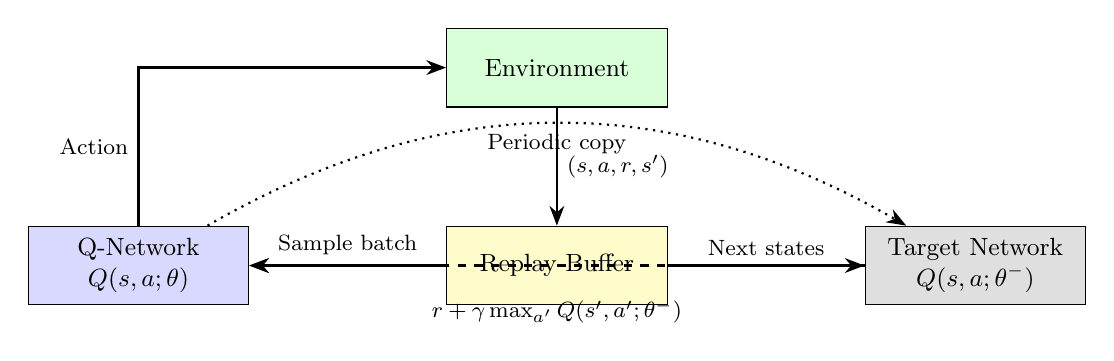
\begin{tikzpicture}[
    node distance=1.5cm,
    block/.style={rectangle, draw, minimum width=2.8cm, minimum height=1cm, align=center, font=\small},
    arrow/.style={-{Stealth[length=2.5mm]}, thick}
]
    % Environment
    \node[block, fill=green!15] (env) {Environment};

    % Replay Buffer (below environment)
    \node[block, fill=yellow!20, below=of env] (buffer) {Replay Buffer};

    % Q-Network (left of buffer)
    \node[block, fill=blue!15, left=2.5cm of buffer] (qnet) {Q-Network\\$Q(s,a;\theta)$};

    % Target Network (right of buffer)
    \node[block, fill=gray!25, right=2.5cm of buffer] (target) {Target Network\\$Q(s,a;\theta^-)$};

    % Arrows showing the flow
    % Environment to buffer
    \draw[arrow] (env) -- node[right, font=\footnotesize] {$(s,a,r,s')$} (buffer);

    % Buffer to Q-network (sample)
    \draw[arrow] (buffer) -- node[above, font=\footnotesize] {Sample batch} (qnet);

    % Buffer to Target (for computing targets)
    \draw[arrow] (buffer) -- node[above, font=\footnotesize] {Next states} (target);

    % Target to Q-network (TD target)
    \draw[arrow, dashed] (target) -- node[below, font=\footnotesize, yshift=-0.3cm] {$r + \gamma \max_{a'} Q(s',a';\theta^-)$} (qnet);

    % Q-network back to environment (action selection)
    \draw[arrow] (qnet) |- node[near start, left, font=\footnotesize] {Action} (env);

    % Periodic update from Q to Target
    \draw[arrow, dotted, thick] (qnet) to[bend left=30] node[below, font=\footnotesize] {Periodic copy} (target);

\end{tikzpicture}
\caption{DQN training loop: experiences are stored in replay buffer, sampled for training, with target network providing stable Q-value targets.}
\label{fig:dqn}
\end{figure}

Table \ref{tab:dqn_variants} summarizes the DQN variants and their key improvements.

\begin{table}[H]
\centering
\caption{DQN Variants and Improvements}
\label{tab:dqn_variants}
\renewcommand{\arraystretch}{1.5}
\begin{tabular*}{\textwidth}{@{\extracolsep{\fill}}p{1.5cm}p{5cm}p{7cm}@{}}
\toprule
\textbf{Variant} & \textbf{Description} & \textbf{Key Equation} \\
\midrule
DQN & Base algorithm with experience replay and target network & $L(\theta) = \mathbb{E}[(r + \gamma \max_{a'} Q(s',a';\theta^-) - Q(s,a;\theta))^2]$ \\
Double & Decouples action selection from evaluation to reduce overestimation bias & $a^* = \arg\max_a Q(s',a;\theta)$, evaluate with $Q(s',a^*;\theta^-)$ \\
Dueling & Separates Q-function into value and advantage streams & $Q(s,a) = V(s) + A(s,a) - \frac{1}{|\mathcal{A}|}\sum_{a'} A(s,a')$ \\
PER & Samples transitions by TD error magnitude for focused learning & Priority $p_i = |\delta_i| + \epsilon$ \\
Noisy & Adds learnable noise to network weights for exploration & $y = (b + Wz)x$ where $z \sim \mathcal{N}(0,1)$ \\
Rainbow & Combines all improvements: Double, Dueling, PER, Noisy, N-step, Distributional & All of the above + distributional $Q(s,a) \sim \mathcal{Z}$ \\
\bottomrule
\end{tabular*}
\renewcommand{\arraystretch}{1.0}
\end{table}

\subsection{Policy Gradient Methods}

While value-based methods learn a value function and derive a policy from it, policy gradient methods directly parameterize and optimize the policy $\pi_\theta(a|s)$. The objective is to maximize the expected return:
\begin{equation}
J(\theta) = \mathbb{E}_{\tau \sim \pi_\theta}[G(\tau)]
\end{equation}

The policy gradient theorem \cite{williams1992simple} provides a way to compute gradients of this objective:
\begin{equation}
\nabla_\theta J(\theta) = \mathbb{E}_{\tau \sim \pi_\theta}\left[\sum_{t=0}^T \nabla_\theta \log \pi_\theta(a_t|s_t) G_t\right]
\end{equation}

The \textbf{REINFORCE} algorithm uses Monte Carlo estimation of this gradient, updating parameters after each complete episode. To reduce variance, a baseline $b(s_t)$ is subtracted from the return, with the state-value function $V(s_t)$ being a common choice. This leads to the advantage function $A(s,a) = Q(s,a) - V(s)$, which measures how much better an action is compared to the average.

\textbf{Actor-Critic} methods combine value-based and policy-based approaches. The actor (policy network) selects actions while the critic (value network) evaluates them, providing lower-variance gradient estimates. The \textbf{Advantage Actor-Critic (A2C)} algorithm \cite{mnih2016asynchronous} uses the TD error as an estimate of the advantage:
\begin{equation}
A(s_t, a_t) \approx r_{t+1} + \gamma V(s_{t+1}) - V(s_t)
\end{equation}

\textbf{Proximal Policy Optimization (PPO)} \cite{schulman2017proximal} has become one of the most popular RL algorithms due to its simplicity and effectiveness. Building on Trust Region Policy Optimization (TRPO) \cite{schulman2015trust}, PPO constrains policy updates to prevent large, destabilizing changes using a clipped surrogate objective:
\begin{equation}
L^{CLIP}(\theta) = \mathbb{E}_t\left[\min\left(r_t(\theta)A_t, \text{clip}(r_t(\theta), 1-\epsilon, 1+\epsilon)A_t\right)\right]
\end{equation}
where $r_t(\theta) = \frac{\pi_\theta(a_t|s_t)}{\pi_{\theta_{old}}(a_t|s_t)}$ is the probability ratio. The clipping prevents the policy from changing too drastically in a single update. PPO also uses Generalized Advantage Estimation (GAE) \cite{schulman2016high} to balance bias and variance in advantage estimates:
\begin{equation}
A_t^{GAE} = \sum_{l=0}^{\infty} (\gamma\lambda)^l \delta_{t+l}
\end{equation}
where $\delta_t = r_t + \gamma V(s_{t+1}) - V(s_t)$ is the TD error and $\lambda$ controls the trade-off.

\begin{figure}[H]
\centering
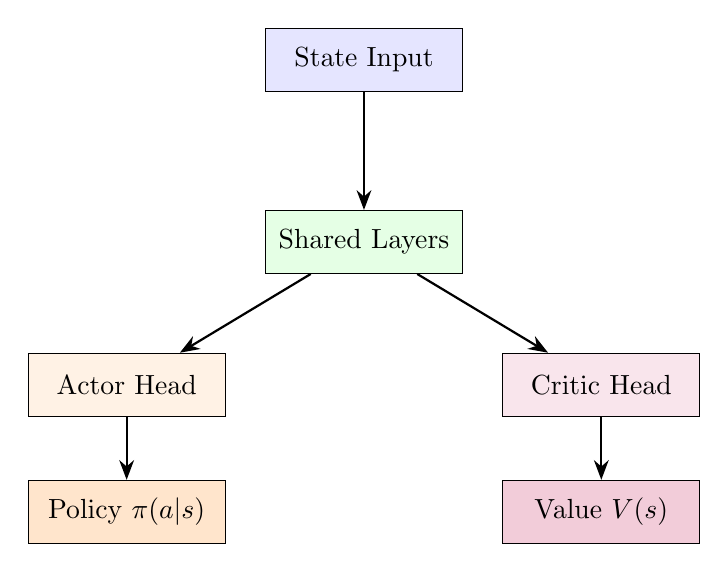
\begin{tikzpicture}[
    node distance=1.5cm,
    block/.style={rectangle, draw, minimum width=2.5cm, minimum height=0.8cm, align=center},
    arrow/.style={-{Stealth[length=2.5mm]}, thick}
]
    % Input
    \node[block, fill=blue!10] (input) {State Input};

    % Shared layers
    \node[block, fill=green!10, below=of input] (shared) {Shared Layers};

    % Actor branch
    \node[block, fill=orange!10, below left=1cm and 0.5cm of shared] (actor) {Actor Head};
    \node[block, fill=orange!20, below=0.8cm of actor] (policy) {Policy $\pi(a|s)$};

    % Critic branch
    \node[block, fill=purple!10, below right=1cm and 0.5cm of shared] (critic) {Critic Head};
    \node[block, fill=purple!20, below=0.8cm of critic] (value) {Value $V(s)$};

    % Arrows
    \draw[arrow] (input) -- (shared);
    \draw[arrow] (shared) -- (actor);
    \draw[arrow] (shared) -- (critic);
    \draw[arrow] (actor) -- (policy);
    \draw[arrow] (critic) -- (value);

\end{tikzpicture}
\caption{Actor-Critic architecture with shared layers, used in PPO and A2C.}
\label{fig:actor_critic}
\end{figure}

Table \ref{tab:policy_gradient_methods} summarizes the policy gradient methods we consider.

\begin{table}[H]
\centering
\caption{Policy Gradient Methods Comparison}
\label{tab:policy_gradient_methods}
\renewcommand{\arraystretch}{1.5}
\begin{tabular*}{\textwidth}{@{\extracolsep{\fill}}p{2cm}p{4.5cm}p{7cm}@{}}
\toprule
\textbf{Method} & \textbf{Description} & \textbf{Key Equation} \\
\midrule
REINFORCE & Monte Carlo policy gradient with episode returns & $\nabla J = \mathbb{E}[\sum_t \nabla \log \pi(a_t|s_t) G_t]$ \\
A2C & Advantage Actor-Critic with TD advantage estimation & $A(s_t,a_t) = r_{t+1} + \gamma V(s_{t+1}) - V(s_t)$ \\
PPO & Clipped surrogate objective for stable updates & $L = \min(r_t A_t, \text{clip}(r_t, 1\pm\epsilon) A_t)$ \\
TRPO & Trust region constraint on policy updates & $\max_\theta J(\theta)$ s.t. $D_{KL}(\pi_{\theta_{old}} || \pi_\theta) \leq \delta$ \\
\bottomrule
\end{tabular*}
\renewcommand{\arraystretch}{1.0}
\end{table}

%==============================================================================
% SECTION 3: IMPLEMENTATION
%==============================================================================
\section{Implementation}

This section describes our implementation of the Snake game environments and reinforcement learning infrastructure. We detail the code structure, GPU vectorization for efficient training, state representations, and action space design.

\subsection{Code Structure}

Our implementation follows a modular architecture organized into several components. The \texttt{core/} directory contains core modules including environments, neural networks, state representations, and utilities. Training scripts for each algorithm (DQN, PPO, A2C) reside in \texttt{scripts/training/}, while \texttt{scripts/visualizer/} provides visualization and recording tools. The \texttt{results/} directory stores trained weights, training data, and generated figures.

All environments follow the Gymnasium (OpenAI Gym) API standard, ensuring compatibility with standard RL libraries. The single-snake environment features a configurable grid (default $10 \times 10$) where the snake starts with length 3 at the center. Food appears randomly on empty cells, and episodes terminate upon collision with walls or the snake's body, or after a timeout of $2 \times \text{grid\_area}$ steps without collecting food.

For competitive scenarios, we implemented a two-snake environment where both snakes share the grid and compete for food. A round ends when one snake reaches a target food count or when a snake dies. The two-snake environment supports both classic (CPU-based) and vectorized (GPU-accelerated) implementations.

\subsection{GPU Vectorization}

A key contribution of our implementation is GPU-accelerated vectorized environments using PyTorch tensors. Instead of running a single game sequentially, we run 128-256 simultaneous games in parallel on the GPU. All game state (snake positions, food locations, directions) is stored as batched tensors, and game logic (collision detection, movement, reward computation) is implemented using vectorized tensor operations.

This vectorization achieves \textbf{100-300x speedup} compared to sequential CPU training. Sequential CPU execution processes approximately 50 episodes per minute, while vectorized GPU training with 256 environments reaches approximately 10,000 episodes per minute. This speedup enables extensive hyperparameter searches and longer training runs that would be infeasible with sequential training. Training 2,000 PPO episodes with 256 parallel environments completes in approximately 3 minutes on an RTX 4070.

\subsection{State Representations}

State representation significantly impacts learning efficiency and final performance. We designed multiple representations with increasing sophistication, ranging from basic 11-dimensional feature vectors to comprehensive 24-dimensional representations.

The simplest representation uses 11 dimensions capturing immediate spatial awareness. This includes three binary danger indicators for collision risk in relative directions (straight, right, left), four binary food direction indicators showing whether food lies up, right, down, or left relative to the head, and four one-hot encoded features representing the snake's current absolute direction. This basic representation provides sufficient information for learning fundamental navigation skills.

Building on this foundation, we developed a 14-dimensional representation that adds flood-fill features. These three additional features measure the ratio of reachable cells in each relative direction using a breadth-first traversal similar to BFS. By computing how much free space is accessible from potential next positions, the agent can avoid moves leading to dead-ends or self-trapping situations. The flood-fill computation normalizes values by the maximum possible free cells, producing features in the range [0, 1].

Further extensions include a 19-dimensional selective representation that adds tail-related features (direction to tail and normalized distance), helping the snake follow its tail for safety in dense configurations. The most comprehensive 24-dimensional enhanced representation adds escape route counts, tail reachability via flood-fill, and snake length ratio. While providing rich information, this representation incurs higher computational cost that may not justify the marginal performance improvement.

For CNN-based approaches, we use a grid representation with 3 channels encoding head position, body position, and food position respectively. This raw grid input requires convolutional layers to extract spatial features but provides complete spatial information without hand-crafted feature engineering.

For competitive two-snake scenarios, we designed a 35-dimensional competitive representation. This combines self-awareness features (danger, food direction, current direction, flood-fill), opponent-awareness features (opponent body danger, head position relative to self, opponent direction, opponent length, distance to opponent, threat level), and competitive metrics (length difference, food count difference, food proximity advantage, space control ratio).

\begin{figure}[H]
\centering
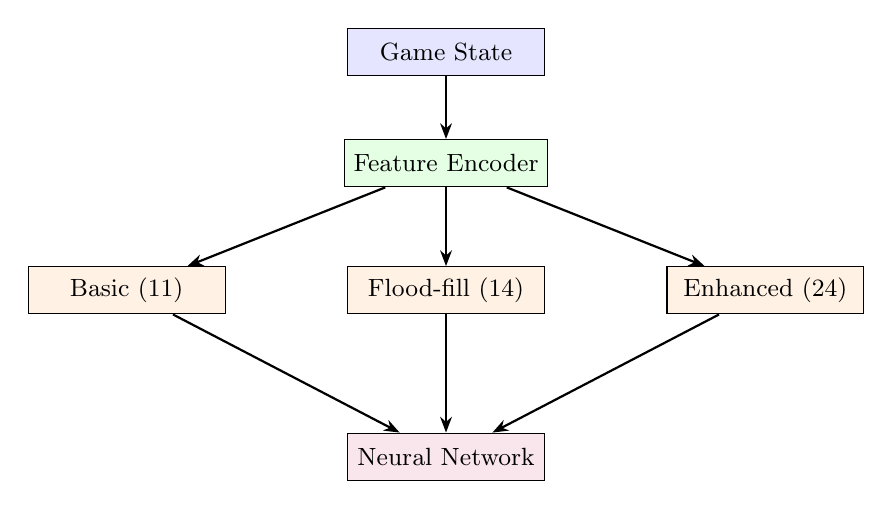
\begin{tikzpicture}[
    node distance=0.8cm,
    box/.style={rectangle, draw, minimum width=2.5cm, minimum height=0.6cm, align=center, font=\small},
    arrow/.style={-{Stealth[length=2mm]}, thick}
]
    % State input
    \node[box, fill=blue!10] (state) {Game State};

    % Encoder
    \node[box, fill=green!10, below=of state] (encoder) {Feature Encoder};

    % Features - increased horizontal spacing
    \node[box, fill=orange!10, below left=1cm and 1.5cm of encoder] (basic) {Basic (11)};
    \node[box, fill=orange!10, below=1cm of encoder] (flood) {Flood-fill (14)};
    \node[box, fill=orange!10, below right=1cm and 1.5cm of encoder] (enhanced) {Enhanced (24)};

    % Network
    \node[box, fill=purple!10, below=1.5cm of flood] (network) {Neural Network};

    \draw[arrow] (state) -- (encoder);
    \draw[arrow] (encoder) -- (basic);
    \draw[arrow] (encoder) -- (flood);
    \draw[arrow] (encoder) -- (enhanced);
    \draw[arrow] (basic) -- (network);
    \draw[arrow] (flood) -- (network);
    \draw[arrow] (enhanced) -- (network);

\end{tikzpicture}
\caption{State representation pipeline with different feature extraction options.}
\label{fig:state_rep}
\end{figure}

\subsection{Action Space}

The action space uses relative directions rather than absolute directions:

\begin{itemize}
\item \textbf{STRAIGHT (0)}: Continue in the current direction
\item \textbf{RIGHT\_TURN (1)}: Turn 90 degrees clockwise
\item \textbf{LEFT\_TURN (2)}: Turn 90 degrees counter-clockwise
\end{itemize}

This relative action space offers several advantages over absolute directions (UP, DOWN, LEFT, RIGHT):

\begin{enumerate}
\item \textbf{Reduced action space}: 3 actions instead of 4, simplifying the learning problem
\item \textbf{No invalid actions}: 180-degree turns (instant death) are impossible by construction
\item \textbf{Direction invariance}: The agent learns behaviors that generalize across all orientations
\end{enumerate}

The relative encoding means the agent's decision depends only on what lies ahead, to the right, and to the left, not on absolute compass directions. This invariance reduces the effective state space the agent must learn.

\subsection{Reward Shaping}

The reward function guides learning behavior. For single-snake, we use food consumption (+10), collision/death (-10), and time penalty (-0.01 per step). The time penalty provides dense feedback encouraging efficient food collection rather than aimless wandering. Some experiments include distance-based shaping ($\pm 1$ for moving toward/away from food) to accelerate early learning.

For competitive two-snake, rewards are more complex. Food consumption gives +10, death results in -50 to -100 depending on configuration, winning the round yields +100, and the opponent dying while the agent survives provides +50. The step penalty is reduced or removed to focus on strategic play rather than speed.

\subsection{Network Architectures}

We implement two network architectures: MLP for feature-based inputs and CNN for grid-based inputs.

\noindent\textbf{MLP Architecture.} For MLP-based agents (feature input), we use two hidden layers with 128 neurons each and ReLU activations. Larger networks (256x256) are used for competitive scenarios requiring more capacity. The output layer produces Q-values (for DQN) or action logits (for policy gradient methods).

\begin{figure}[H]
\centering
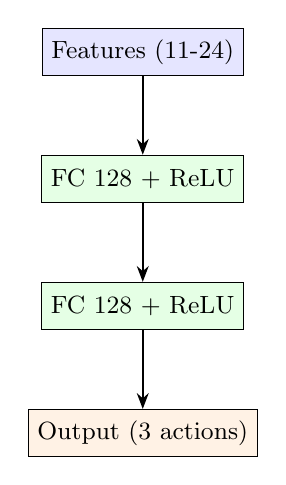
\begin{tikzpicture}[
    node distance=1cm,
    layer/.style={rectangle, draw, minimum width=2.5cm, minimum height=0.6cm, align=center, font=\small},
    arrow/.style={-{Stealth[length=2mm]}, thick}
]
    \node[layer, fill=blue!10] (input) {Features (11-24)};
    \node[layer, fill=green!10, below=of input] (fc1) {FC 128 + ReLU};
    \node[layer, fill=green!10, below=of fc1] (fc2) {FC 128 + ReLU};
    \node[layer, fill=orange!10, below=of fc2] (output) {Output (3 actions)};

    \draw[arrow] (input) -- (fc1);
    \draw[arrow] (fc1) -- (fc2);
    \draw[arrow] (fc2) -- (output);
\end{tikzpicture}
\caption{MLP architecture for feature-based state input.}
\label{fig:mlp_arch}
\end{figure}

\noindent\textbf{CNN Architecture.} For CNN-based agents (grid input), we use three convolutional layers (32, 64, 64 filters with 3x3 kernels), followed by a fully connected layer (256 neurons) and the output layer. Padding preserves spatial dimensions through the convolutional layers.

\begin{figure}[H]
\centering
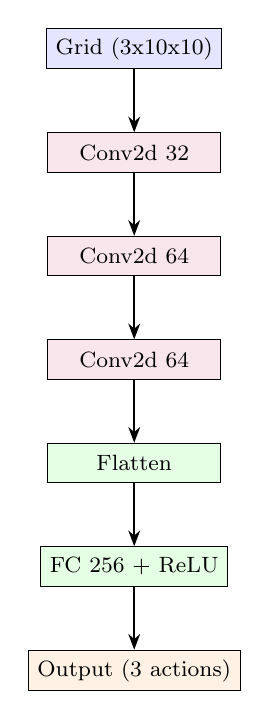
\begin{tikzpicture}[
    node distance=0.8cm,
    layer/.style={rectangle, draw, minimum width=2.2cm, minimum height=0.5cm, align=center, font=\footnotesize},
    arrow/.style={-{Stealth[length=2mm]}, thick}
]
    \node[layer, fill=blue!10] (input) {Grid (3x10x10)};
    \node[layer, fill=purple!10, below=of input] (conv1) {Conv2d 32};
    \node[layer, fill=purple!10, below=of conv1] (conv2) {Conv2d 64};
    \node[layer, fill=purple!10, below=of conv2] (conv3) {Conv2d 64};
    \node[layer, fill=green!10, below=of conv3] (flatten) {Flatten};
    \node[layer, fill=green!10, below=of flatten] (fc) {FC 256 + ReLU};
    \node[layer, fill=orange!10, below=of fc] (output) {Output (3 actions)};

    \draw[arrow] (input) -- (conv1);
    \draw[arrow] (conv1) -- (conv2);
    \draw[arrow] (conv2) -- (conv3);
    \draw[arrow] (conv3) -- (flatten);
    \draw[arrow] (flatten) -- (fc);
    \draw[arrow] (fc) -- (output);
\end{tikzpicture}
\caption{CNN architecture for grid-based state input.}
\label{fig:cnn_arch}
\end{figure}

Although CNNs are well-suited for spatial feature detection and could theoretically scale better to larger grid sizes by leveraging GPU parallelism for convolution operations, in practice CNNs are slower to run than MLPs with hand-crafted features. The convolutional operations add computational overhead that outweighs their benefits for our relatively small $10 \times 10$ grid. For this problem size, the MLP with flood-fill features provides both better performance and faster inference.

PPO uses separate actor and critic networks, or a shared backbone with separate heads. The actor outputs action logits processed through softmax for action probabilities. The critic outputs a single scalar value estimate.

\subsection{Baseline Algorithms}

To contextualize RL agent performance, we implemented several deterministic baseline algorithms. The random baseline selects actions uniformly at random, providing a lower bound on expected performance. The greedy food baseline uses A* pathfinding to navigate toward the nearest food, representing a simple but effective heuristic. The shortest path baseline employs Dijkstra's algorithm considering both walls and the snake's body as obstacles, representing near-optimal navigation when sufficient free space exists. These baselines establish performance benchmarks against which learning algorithms can be compared.

\subsection{Training Procedures}

We implemented training scripts for all algorithms with consistent interfaces and configurable hyperparameters. Table \ref{tab:hyperparameters} summarizes key hyperparameters.

\begin{table}[H]
\centering
\caption{Training Hyperparameters}
\label{tab:hyperparameters}
\begin{tabular}{lcc}
\toprule
\textbf{Parameter} & \textbf{DQN} & \textbf{PPO} \\
\midrule
Learning rate & 0.001 & 0.0003 \\
Discount factor ($\gamma$) & 0.99 & 0.99 \\
Batch size & 64 & 64 \\
Buffer/Rollout size & 100,000 & 2,048 \\
Hidden layers & 128x128 & 128x128 \\
$\epsilon$ start/end & 1.0/0.01 & N/A \\
$\epsilon$ decay & 0.995 & N/A \\
Clip parameter & N/A & 0.2 \\
GAE $\lambda$ & N/A & 0.95 \\
Entropy coefficient & N/A & 0.01 \\
Target update freq & 1,000 steps & N/A \\
\bottomrule
\end{tabular}
\end{table}

For DQN variants, we train for 5,000-10,000 episodes with 256 parallel environments. Training uses Adam optimizer with gradient clipping (max norm 1.0). The replay buffer stores transitions and samples uniformly (or by priority for PER). The target network updates every 1,000 training steps.

For policy gradient methods, we collect rollouts of 2,048 steps across parallel environments, then perform multiple epochs (4-10) of mini-batch updates. PPO uses the clipped objective with value function and entropy bonuses. A2C uses simpler advantage estimation without clipping.

For two-snake curriculum training, we progress through five stages with increasing opponent difficulty. Each stage trains until a win rate threshold is achieved (70\% for static, 60\% for random, 55\% for greedy, 50\% for frozen) or a maximum step count is reached. The final co-evolution stage trains both agents simultaneously.

%==============================================================================
% SECTION 4: EXPERIMENTS
%==============================================================================
\section{Experiments}

This section presents our experimental results, organized to demonstrate the progression of our investigation. We begin with vanilla implementations of DQN and PPO, then explore DQN variants and advanced algorithms. We investigate death causes to understand failure modes, introduce flood-fill features as a solution, study reward system modifications, and demonstrate grid size generalization. Finally, we present results from the competitive two-snake environment.

\subsection{Vanilla DQN and PPO}

We first establish baseline performance with standard implementations of DQN and PPO using basic features (danger indicators, food direction, current direction). Both algorithms were trained with 256 parallel environments on a $10 \times 10$ grid. DQN was trained for 3,000 episodes, while PPO achieved comparable results in 2,000 episodes due to its superior sample efficiency.

Figure \ref{fig:dqn_results} shows DQN training progression with basic features, demonstrating the characteristic learning curve with initial exploration phase followed by exploitation. Figure \ref{fig:ppo_results} shows PPO training, which exhibits faster convergence and more stable learning dynamics.

\begin{figure}[H]
\centering
\includegraphics[width=0.95\textwidth]{dqn_basic_scores.png}
\caption{DQN training with basic features. Episode scores plateau around 16-17 average with maximum score of 31. Without spatial awareness features, performance is limited by frequent entrapment deaths.}
\label{fig:dqn_results}
\end{figure}

\begin{figure}[H]
\centering
\includegraphics[width=0.95\textwidth]{ppo_basic_scores.png}
\caption{PPO training with basic features. Despite faster convergence, basic features limit performance to around 17-18 average with maximum score of 35, similar to DQN.}
\label{fig:ppo_results}
\end{figure}

PPO consistently outperforms DQN in sample efficiency, achieving comparable or better final scores in fewer episodes. This advantage stems from PPO's on-policy learning with entropy regularization, which maintains exploration throughout training, unlike DQN's decaying epsilon-greedy strategy.

\subsection{DQN Variants}

We evaluated several DQN improvements to understand their individual contributions:

\begin{itemize}
\item \textbf{Double DQN}: Reduces overestimation bias by decoupling action selection from evaluation
\item \textbf{Dueling DQN}: Separates value and advantage streams for better state evaluation
\item \textbf{Prioritized Experience Replay (PER)}: Focuses learning on high-error transitions
\item \textbf{Noisy Networks}: Replaces epsilon-greedy with learnable exploration
\end{itemize}

In our experiments, Double DQN provided the most consistent improvement, reducing Q-value overestimation that can destabilize learning. Dueling DQN showed benefits in states where most actions have similar value. PER accelerated early learning but required careful tuning of priority parameters. Noisy networks eliminated the need for epsilon scheduling but required longer training to learn appropriate exploration levels.

\noindent\textbf{Rainbow DQN.} Rainbow DQN \cite{hessel2018rainbow} combines multiple DQN improvements into a single agent: Double Q-learning for reduced overestimation, Dueling architecture for better value estimation, Prioritized Experience Replay for efficient sampling, Noisy networks for exploration, and Distributional RL for modeling return distributions. Our implementation uses 51 atoms with support range [-20, 500] to capture the full reward distribution. In our experiments, Rainbow DQN achieves the highest average score of 37.54, outperforming all individual DQN variants. The combination proves synergistic: while individual improvements yield modest gains (22-30 avg score), their combination achieves 63\% improvement over standard DQN.

\subsection{Death Cause Investigation}

Understanding why agents die provides insight into failure modes and guides improvements. We categorize deaths into three types:

\begin{itemize}
\item \textbf{Wall collisions}: Hitting the grid boundary
\item \textbf{Self-collisions}: Hitting the snake's own body during normal movement
\item \textbf{Entrapments}: The snake boxes itself in with no valid escape moves
\end{itemize}

\noindent\textbf{Cumulative Death Curves.} The right panels of Figures \ref{fig:dqn_results} and \ref{fig:ppo_results} show cumulative death causes over training episodes. These curves visualize how death causes shift as the agent learns, with entrapment typically dominating early before the agent develops spatial awareness.

With basic features, entrapment is the dominant death cause at 74-82\% of deaths. This indicates that agents without spatial awareness frequently maneuver into positions from which escape is impossible. The remaining deaths split between wall and self-collisions, often occurring during aggressive food pursuit.

\subsection{Flood-Fill Feature Engineering}

The flood-fill feature addresses the entrapment problem by giving the agent spatial awareness about reachable free space. For each potential next position, we compute the ratio of cells reachable via flood-fill traversal.

\noindent\textbf{Algorithm.} The flood-fill computation uses a breadth-first traversal:

\begin{enumerate}
\item Start from the candidate next position
\item Initialize visited set and queue with start position
\item While queue is not empty:
\begin{itemize}
\item Dequeue current cell
\item For each adjacent cell (up, down, left, right):
\item If cell is valid, not visited, and not blocked by snake body: add to visited and enqueue
\end{itemize}
\item Return $|$visited$|$ / max\_free\_cells
\end{enumerate}

The result is a value in [0, 1] representing the fraction of free space reachable from that direction. Low values indicate potential dead-ends; high values indicate open space.

\noindent\textbf{Impact on Performance.} Table \ref{tab:representation_comparison} compares performance with and without flood-fill features. The flood-fill representation consistently doubles average scores compared to basic features, representing the single most impactful improvement in our experiments.

\begin{table}[H]
\centering
\caption{Single-Snake Performance: Basic vs Flood-fill Features}
\label{tab:representation_comparison}
\begin{tabular}{llcccc}
\toprule
\textbf{Algorithm} & \textbf{Features} & \textbf{Episodes} & \textbf{Avg Score} & \textbf{Max Score} & \textbf{Entrap \%} \\
\midrule
DQN & Basic & 5,000 & 16.2 & 35 & 74\% \\
DQN & Flood-fill & 10,000 & 27.1 & 54 & 42\% \\
PPO & Basic & 2,000 & 19.2 & 45 & 82\% \\
PPO & Flood-fill & 2,000 & 37.5 & 64 & 37\% \\
\bottomrule
\end{tabular}
\end{table}

The flood-fill feature provides spatial awareness about which moves lead to open areas versus dead-ends. The impact is most dramatic for avoiding entrapment deaths: with basic features, 74-82\% of deaths are entrapments; with flood-fill, this drops to 37-42\%.

\subsection{Reward System Modification}

We investigated whether reward engineering could reduce deaths beyond what flood-fill achieves. Specifically, we studied the death penalty hyperparameter, testing values from -10 to -100. This parameter controls how strongly the agent is penalized for dying, potentially affecting the exploration-exploitation trade-off and learned risk tolerance.

Table \ref{tab:ppo_basic_penalty} shows PPO results with basic features across death penalties. The penalty has moderate impact, with all values producing similar average scores in the 18-20 range.

\begin{table}[H]
\centering
\caption{PPO Basic Features: Death Penalty Study}
\label{tab:ppo_basic_penalty}
\begin{tabular}{ccc}
\toprule
\textbf{Death Penalty} & \textbf{Avg Score} & \textbf{Max Score} \\
\midrule
-10 & 19.48 & 45 \\
-20 & 18.40 & 45 \\
-30 & 18.25 & 40 \\
-40 & 19.30 & 41 \\
-50 & 19.25 & 40 \\
-100 & 19.93 & 39 \\
\bottomrule
\end{tabular}
\end{table}

Table \ref{tab:ppo_flood_penalty} shows PPO results with flood-fill features. Here we observe consistently higher scores across all penalties, with the -100 penalty producing the best average score of 39.74.

\begin{table}[H]
\centering
\caption{PPO Flood-fill Features: Death Penalty Study}
\label{tab:ppo_flood_penalty}
\begin{tabular}{ccc}
\toprule
\textbf{Death Penalty} & \textbf{Avg Score} & \textbf{Max Score} \\
\midrule
-10 & 35.08 & 59 \\
-20 & 35.91 & 60 \\
-30 & 36.98 & 64 \\
-40 & 37.52 & 59 \\
-50 & 36.76 & 58 \\
-100 & 39.74 & 56 \\
\bottomrule
\end{tabular}
\end{table}

The death penalty has less impact than state representation. Across all tested values, the difference in average score is at most 4-5 points, while switching from basic to flood-fill features provides an 18-point improvement. This suggests that investing effort in state representation design yields greater returns than hyperparameter tuning.

Figures \ref{fig:dqn_flood} and \ref{fig:ppo_flood} demonstrate the dramatic improvement from flood-fill features compared to the basic feature results shown in Figures \ref{fig:dqn_results} and \ref{fig:ppo_results}.

\begin{figure}[H]
\centering
\includegraphics[width=0.95\textwidth]{dqn_flood-fill_scores.png}
\caption{DQN with flood-fill features training scores. With spatial awareness, scores improve dramatically to 24-27 average with maximum score of 53, compared to 16-17 average with basic features. The flood-fill features enable the agent to avoid dead-end positions.}
\label{fig:dqn_flood}
\end{figure}

\begin{figure}[H]
\centering
\includegraphics[width=0.95\textwidth]{ppo_flood-fill_scores.png}
\caption{PPO with flood-fill features training scores. PPO achieves the best performance with 35-37 average score and maximum of 52, compared to 17-18 average with basic features. The combination of PPO's sample efficiency and flood-fill's spatial awareness produces optimal results.}
\label{fig:ppo_flood}
\end{figure}

\subsection{Grid Size Generalization}

A key advantage of our feature-based state representation is grid-size independence. Because the features encode relative spatial information (danger indicators, food direction, flood-fill ratios) rather than absolute positions, an agent trained on a $10 \times 10$ grid can generalize to larger or smaller grids without retraining.

To validate this, we trained a DQN agent with flood-fill features on a $10 \times 10$ grid for 5,000 episodes, then evaluated its performance on $8 \times 8$, $10 \times 10$, $15 \times 15$, and $20 \times 20$ grids without any additional training. Table \ref{tab:grid_generalization} summarizes the results.

\begin{table}[H]
\centering
\caption{Grid Size Generalization: Model Trained on 10x10, Evaluated on Multiple Sizes}
\label{tab:grid_generalization}
\begin{tabular}{lcccc}
\toprule
\textbf{Grid Size} & \textbf{Avg Score} & \textbf{Max Score} & \textbf{Theoretical Max} & \textbf{\% of Max} \\
\midrule
$8 \times 8$ & 25.1 & 39 & 61 & 41.2\% \\
$10 \times 10$ (trained) & 34.8 & 54 & 97 & 35.9\% \\
$15 \times 15$ & 57.1 & 72 & 222 & 25.7\% \\
$20 \times 20$ & 55.2 & 71 & 397 & 13.9\% \\
\bottomrule
\end{tabular}
\end{table}

The results demonstrate successful generalization across grid sizes. Absolute scores actually increase on larger grids because the snake has more room to maneuver before facing space constraints. The percentage of theoretical maximum decreases for larger grids, which is expected since filling a larger grid requires longer survival and more strategic planning.

\begin{figure}[H]
\centering
\includegraphics[width=0.95\textwidth]{grid_size_generalization.png}
\caption{Grid size generalization results. Left: Average scores increase with grid size due to more maneuvering room. Right: Performance relative to theoretical maximum decreases for larger grids. The model trained on 10x10 (blue) successfully transfers to other grid sizes (green).}
\label{fig:grid_generalization}
\end{figure}

The feature encoder only requires normalizing flood-fill values by the new grid's maximum free cells. All other features (danger indicators, food direction, current direction) remain unchanged, enabling zero-shot transfer to unseen grid sizes.

\subsection{Two-Snake Competitive Environment}

Competitive training proved more challenging than single-snake scenarios, requiring curriculum learning for stable performance. In the two-snake environment, both agents share the grid and compete for food, introducing non-stationarity as each agent's policy evolves during training.

\noindent\textbf{Network Size Investigation.} We investigate whether larger networks produce better competitive agents. We train two agents with different network capacities:

\begin{itemize}
\item \textbf{Big network}: 256x256 hidden layers (131,000+ parameters)
\item \textbf{Small network}: 128x128 hidden layers (33,000+ parameters)
\end{itemize}

The hypothesis is that competitive scenarios require more representational capacity to model opponent behavior, strategic planning, and multi-objective optimization (food collection vs. survival vs. blocking opponent).

\noindent\textbf{Expected Challenges.} Competitive multi-agent RL introduces several challenges absent in single-agent settings:

\begin{enumerate}
\item \textbf{Non-stationarity}: The opponent's policy changes during training, violating the stationarity assumption of most RL algorithms
\item \textbf{Credit assignment}: When one snake dies, it is unclear whether this resulted from its own mistake or the opponent's skill
\item \textbf{Reward design}: Balancing food collection, survival, and competitive objectives requires careful reward engineering
\item \textbf{Exploration collapse}: Both agents may converge to avoiding each other rather than competing
\end{enumerate}

\noindent\textbf{Naive Attempt: Direct Co-evolution.} Our initial approach was direct co-evolution: training both agents simultaneously from random initialization. This approach failed to produce capable agents. Both snakes learned to avoid the center of the grid and each other, resulting in passive play with neither agent collecting food efficiently.

The failure occurs because early in training, random policies cause frequent collisions. The agents learn that approaching the opponent is dangerous, but this learned avoidance prevents them from developing competitive food-collection strategies.

\noindent\textbf{Curriculum Learning.} To address co-evolution failure, we employ a five-stage curriculum with progressively increasing opponent difficulty. Table \ref{tab:curriculum_stages} summarizes the curriculum design.

\begin{table}[H]
\centering
\caption{Curriculum Learning Stages}
\label{tab:curriculum_stages}
\begin{tabular}{clcccc}
\toprule
\textbf{Stage} & \textbf{Opponent} & \textbf{Min Steps} & \textbf{Win Rate} & \textbf{Target Food} & \textbf{Agent2 Trains} \\
\midrule
0 & Static & 5,000 & 70\% & 10 & No \\
1 & Random & 7,500 & 60\% & 10 & No \\
2 & Greedy & 10,000 & 55\% & 4 & No \\
3 & Frozen Policy & 10,000 & 50\% & 6 & No \\
4 & Co-evolution & 20,000 & N/A & 8 & Yes \\
\bottomrule
\end{tabular}
\end{table}

Each stage requires achieving both the minimum training steps and the win rate threshold before advancing. The target food count decreases in middle stages to encourage faster rounds and more learning signal.

\noindent\textbf{Curriculum Results.} \textit{[PLACEHOLDER: Results table showing performance metrics at each curriculum stage]}

\begin{table}[H]
\centering
\caption{Curriculum Learning Results by Stage}
\label{tab:curriculum_results}
\begin{tabular}{lcccc}
\toprule
\textbf{Stage} & \textbf{Win Rate} & \textbf{Avg Score} & \textbf{Steps to Threshold} & \textbf{Time (min)} \\
\midrule
Stage 0 (Static) & -- & -- & -- & -- \\
Stage 1 (Random) & -- & -- & -- & -- \\
Stage 2 (Greedy) & -- & -- & -- & -- \\
Stage 3 (Frozen) & -- & -- & -- & -- \\
Stage 4 (Co-evolution) & -- & -- & -- & -- \\
\bottomrule
\end{tabular}
\end{table}

\noindent\textbf{Final Competition: Big vs Small Network.} After curriculum training, we pit the big network (256x256) against the small network (128x128) in head-to-head competition to evaluate whether network capacity translates to competitive advantage.

\textit{[PLACEHOLDER: Final competition results - win rates, average scores, and qualitative observations about playing styles]}

Key observations from competitive training include:

\begin{itemize}
\item Direct co-evolution often fails, as both snakes learn avoidance rather than competition
\item Curriculum learning produces more capable agents by building skills incrementally
\item Asymmetric network sizes (larger network for the main agent) improve training stability
\item Victory rewards (+100) and death penalties (-50 to -100) are essential for competitive behavior
\end{itemize}

The curriculum approach allows agents to first master basic navigation and food collection before facing adaptive opponents, resulting in more robust competitive strategies.

%==============================================================================
% SECTION 5: DISCUSSION
%==============================================================================
\section{Discussion}

This section analyzes experimental results, organizing findings to match our experimental progression.

\subsection{Algorithm Comparison}

Our comprehensive evaluation across seven algorithms (see Appendix \ref{app:algorithm_comparison} for full details) reveals that PPO achieves the highest average score (19.51) with basic features, outperforming all DQN variants which cluster around 15-17 average score. Dueling DQN (16.70) and Rainbow DQN (16.49) show modest improvements over standard DQN (15.32).

PPO learns faster and achieves more stable performance compared to value-based methods. In wall-clock time, DQN trains significantly faster due to its simpler update mechanism: while PPO requires multiple epochs of mini-batch updates per rollout, DQN performs single-step updates from replay buffer samples. For rapid prototyping, DQN offers quicker iteration cycles.

Individual DQN variants show modest improvements with basic features: Dueling DQN provides the best value-based performance; Double DQN reduces overestimation but shows similar final scores; PER and Noisy networks provide marginal benefits. Rainbow DQN's combination of improvements does not provide the dramatic gains seen in other domains, likely because the entrapment problem (70-90\% of deaths) cannot be solved through better value estimation alone.

\subsection{State Representation Impact}
\label{sec:representation_comparison}

The flood-fill feature emerges as the most impactful state representation enhancement, nearly doubling average scores. PPO with basic features achieves 19.2 average score, while PPO with flood-fill achieves 37.5, a 95\% improvement. By measuring reachable free space in each direction, flood-fill enables the agent to avoid moves leading to dead-ends.

CNN-based approaches consistently underperform MLP-based approaches with feature engineering. This suggests that hand-crafted features capturing spatial relationships provide more relevant information than raw grid inputs for this relatively small-scale problem. CNNs may show advantages for larger grids or more complex visual environments.

\subsection{Death Cause Analysis}

Death cause categorization reveals fundamental differences between representations. With basic features, entrapment accounts for 74-82\% of deaths because the snake boxes itself in without escape routes. With flood-fill features, entrapment drops to 37-42\%, while wall and self-collision deaths increase proportionally.

This shift from strategic to tactical deaths represents a more robust learned policy. Flood-fill agents actively avoid self-trapping situations, dying instead from momentary navigation errors rather than strategic dead-ends.

\subsection{Reward Engineering Insights}

Our hyperparameter study across six death penalties (-10 to -100) shows at most 4-5 point variation in average score within each representation type. The death penalty affects learned risk tolerance but does not fundamentally change agent capability.

This contrasts with state representation, where the basic-to-flood-fill change provides an 18-point improvement. The finding suggests that for spatial planning problems, investing in state representation design yields greater returns than hyperparameter tuning.

Sparse rewards (only receiving signal upon eating food or dying) slow early learning. Distance-based reward shaping ($\pm 1$ for moving toward/away from food) accelerates initial progress but must be carefully scaled to avoid distorting the optimal policy.

\subsection{Two-Snake Competition Insights}

Curriculum learning proves essential for competitive scenarios. Direct co-evolution often fails: both snakes learn to avoid each other rather than compete effectively. The staged curriculum allows agents to master basic skills before facing adaptive opponents.

Each stage contributes differently: static opponents teach basic movement, random opponents teach robustness, greedy opponents teach competition, and frozen opponents prevent co-adaptation artifacts. The progression ensures agents develop complete competitive strategies rather than narrow avoidance behaviors.

Two-snake credit assignment remains challenging. When one snake dies, determining whether this resulted from its own mistake or the opponent's skill is ambiguous. Curriculum learning helps by initially removing this ambiguity (against deterministic opponents).

%==============================================================================
% SECTION 6: CONCLUSION
%==============================================================================
\section{Conclusion}

This project comprehensively investigated reinforcement learning techniques applied to the Snake game. We implemented multiple algorithms spanning value-based methods (DQN with Double, Dueling, PER, Noisy, and Rainbow variants) and policy gradient methods (REINFORCE, A2C, PPO), evaluated them in both single-snake and competitive two-snake scenarios, and identified key factors affecting performance.

Our main contributions include implementing GPU-accelerated vectorized environments achieving 100-300x speedup, designing and comparing multiple state representations with flood-fill features proving most impactful, demonstrating that PPO achieves the best performance both with basic features (19.51 avg score) and flood-fill features (37.5 avg score), developing effective curriculum learning strategies for competitive two-snake training, and providing practical recommendations for algorithm and representation selection.

\subsection{Limitations}

Despite achieving reasonable performance, our approach has several limitations:

\begin{itemize}
\item \textbf{Sample inefficiency}: Training requires millions of environment steps to achieve competent play. This is a fundamental limitation of deep RL, as discussed by Alex Irpan in his influential article ``Deep Reinforcement Learning Doesn't Work Yet'' \cite{irpan2018deep}. For context, Rainbow DQN requires approximately 18 million frames (83 hours of gameplay) to achieve human-level performance on Atari games, yet humans master these games in minutes. Earlier methods like Nature DQN required 200 million frames without reaching comparable performance. Even simple simulated robotics tasks in MuJoCo require $10^5$ to $10^7$ steps despite having perfect state information. Figure \ref{fig:sample_inefficiency} illustrates this gap. Our Snake agents face the same challenge: while GPU vectorization helps by parallelizing experience collection, the underlying sample complexity remains high. More sample-efficient approaches (model-based RL, offline RL) could reduce data requirements.

\begin{figure}[H]
\centering
\includegraphics[width=0.95\textwidth]{sample_inefficiency.png}
\caption{Sample inefficiency in deep RL: median human-normalized scores across 57 Atari games. Rainbow DQN reaches human-level performance at 18 million frames. Source: \cite{irpan2018deep}.}
\label{fig:sample_inefficiency}
\end{figure}

\item \textbf{High variance and seed sensitivity}: Different random seeds produce varying results, making reproducibility challenging. Figure \ref{fig:pendulum_variance} shows this phenomenon on the simple Pendulum task: with identical hyperparameters, 3 out of 10 runs fail to learn, while successful runs show substantial variance in convergence time. This instability is common across deep RL and affects our Snake experiments as well; results can vary by 20-30\% across seeds with identical hyperparameters.

\begin{figure}[H]
\centering
\includegraphics[width=0.95\textwidth]{pendulum_results.png}
\caption{High variance in deep RL: 10 independent runs on Pendulum with identical hyperparameters. 3 of 10 runs fail entirely. Source: \cite{irpan2018deep}.}
\label{fig:pendulum_variance}
\end{figure}

\end{itemize}

Beyond these fundamental challenges, hyperparameter sensitivity remains a concern: parameters optimized for one grid size may not transfer to others, and automated hyperparameter search could address this but increases computational costs. However, our grid size generalization experiments demonstrate that feature-based representations transfer well: a model trained on 10x10 achieves 25-57 average scores on grids from 8x8 to 20x20 without retraining (see Table \ref{tab:grid_generalization}). Finally, agents face a maximum score ceiling, as maintaining survival becomes increasingly difficult as the snake grows. Our agents typically plateau at 25-40\% of the theoretical maximum score.

\subsection{Future Directions}

Several promising directions could extend this work. Hierarchical RL could decompose the problem into high-level planning (path to food) and low-level control (collision avoidance), improving both learning efficiency and interpretability. N-step returns and more sophisticated distributional approaches could further enhance Rainbow DQN's already strong performance.

Transfer learning techniques like progressive networks or policy distillation could enable knowledge transfer between grid sizes, while population-based training for competitive scenarios could evolve diverse strategies rather than converging to a single equilibrium, producing more robust agents. Model-based approaches that learn a world model could improve sample efficiency by enabling planning and imagination. Finally, attention mechanisms or graph neural networks could help agents better reason about long-range spatial dependencies as the snake grows.

This work demonstrates that classic games remain valuable testbeds for RL research, providing accessible environments for algorithm development while presenting genuine challenges in state representation, reward design, and training stability.

%==============================================================================
% APPENDIX: ALGORITHM COMPARISON
%==============================================================================
\newpage
\appendix
\section{Algorithm Comparison}
\label{app:algorithm_comparison}

This appendix presents a comprehensive comparison of all implemented reinforcement learning algorithms trained under identical conditions: 3000 episodes, 256 parallel environments, 10x10 grid, basic features (no flood-fill), and fixed random seed for reproducibility.

\subsection{Performance Summary}

Table \ref{tab:appendix_results} summarizes the final performance metrics for each algorithm.

\begin{table}[H]
\centering
\caption{Algorithm Performance Comparison (3000 episodes, basic features)}
\label{tab:appendix_results}
\begin{tabular}{lcccc}
\toprule
\textbf{Algorithm} & \textbf{Avg Score} & \textbf{Max Score} & \textbf{Training Time (s)} & \textbf{Entrapment \%} \\
\midrule
PPO & \textbf{19.51} & \textbf{40} & 563 & 77.5 \\
Dueling DQN & 16.70 & 31 & 140 & 72.5 \\
Rainbow DQN & 16.49 & 32 & 448 & 89.3 \\
PER DQN & 15.99 & 34 & 158 & 71.5 \\
DQN & 15.32 & 33 & 138 & 72.5 \\
Noisy DQN & 15.28 & 34 & 181 & 82.2 \\
Double DQN & 14.79 & 32 & 141 & 72.8 \\
\bottomrule
\end{tabular}
\end{table}

PPO achieves the highest average score (19.51), outperforming all DQN variants. Without flood-fill features, all algorithms plateau around 15-20 average score, significantly lower than the 35-40 scores achieved with flood-fill (see Section \ref{sec:representation_comparison}). This demonstrates that state representation has a larger impact on performance than algorithm choice.

\subsection{Training Curves}

Figure \ref{fig:appendix_training} shows the training score progression for all algorithms. PPO learns fastest and achieves the highest final performance. DQN variants cluster together around 15-17 average score, with Rainbow DQN showing early promise but similar final performance.

\begin{figure}[H]
\centering
\includegraphics[width=0.95\textwidth]{appendix_scores.png}
\caption{Training score curves for all algorithms over 3000 episodes with basic features. PPO achieves the highest performance (~19.5), while DQN variants plateau around 15-17 average score. Without flood-fill features, all algorithms are limited by their inability to detect dead-ends.}
\label{fig:appendix_training}
\end{figure}

\subsection{Death Cause Analysis}

Figure \ref{fig:appendix_deaths} shows the distribution of death causes across algorithms. The dominance of entrapment deaths (70-90\%) across all algorithms highlights the limitation of basic features.

\begin{figure}[H]
\centering
\includegraphics[width=0.95\textwidth]{appendix_deaths.png}
\caption{Death cause distribution by algorithm with basic features. Entrapment (orange) dominates across all algorithms (70-90\%), demonstrating that without flood-fill features, agents cannot detect and avoid dead-ends. Rainbow DQN shows the highest entrapment rate (89.3\%) but lowest wall/self collision rates, indicating it learned to avoid immediate obstacles but still falls into spatial traps.}
\label{fig:appendix_deaths}
\end{figure}

The high entrapment rates across all algorithms demonstrate a fundamental limitation of basic features: agents cannot anticipate spatial dead-ends. While Rainbow DQN and PPO achieve lower wall and self-collision rates (indicating better immediate obstacle avoidance), they still succumb to entrapment at similar rates to simpler algorithms. This motivates the flood-fill feature engineering described in the main text, which reduces entrapment from 70-90\% to 40-55\%.

%==============================================================================
% REFERENCES
%==============================================================================
\newpage
\bibliographystyle{IEEEtran}
\begin{thebibliography}{99}

\bibitem{sutton2018reinforcement}
R.~S. Sutton and A.~G. Barto, \emph{Reinforcement Learning: An Introduction}, 2nd ed. MIT Press, 2018.

\bibitem{mnih2015human}
V.~Mnih \emph{et al.}, ``Human-level control through deep reinforcement learning,'' \emph{Nature}, vol. 518, no. 7540, pp. 529--533, 2015.

\bibitem{silver2016mastering}
D.~Silver \emph{et al.}, ``Mastering the game of Go with deep neural networks and tree search,'' \emph{Nature}, vol. 529, no. 7587, pp. 484--489, 2016.

\bibitem{watkins1992q}
C.~J. Watkins and P.~Dayan, ``Q-learning,'' \emph{Machine Learning}, vol. 8, no. 3-4, pp. 279--292, 1992.

\bibitem{van2016deep}
H.~van Hasselt, A.~Guez, and D.~Silver, ``Deep reinforcement learning with Double Q-learning,'' in \emph{Proc. AAAI Conf. Artificial Intelligence}, 2016.

\bibitem{wang2016dueling}
Z.~Wang \emph{et al.}, ``Dueling network architectures for deep reinforcement learning,'' in \emph{Proc. Int. Conf. Machine Learning}, 2016.

\bibitem{schaul2016prioritized}
T.~Schaul, J.~Quan, I.~Antonoglou, and D.~Silver, ``Prioritized experience replay,'' in \emph{Proc. Int. Conf. Learning Representations}, 2016.

\bibitem{fortunato2018noisy}
M.~Fortunato \emph{et al.}, ``Noisy networks for exploration,'' in \emph{Proc. Int. Conf. Learning Representations}, 2018.

\bibitem{williams1992simple}
R.~J. Williams, ``Simple statistical gradient-following algorithms for connectionist reinforcement learning,'' \emph{Machine Learning}, vol. 8, no. 3-4, pp. 229--256, 1992.

\bibitem{schulman2017proximal}
J.~Schulman, F.~Wolski, P.~Dhariwal, A.~Radford, and O.~Klimov, ``Proximal policy optimization algorithms,'' \emph{arXiv preprint arXiv:1707.06347}, 2017.

\bibitem{schulman2016high}
J.~Schulman, P.~Moritz, S.~Levine, M.~Jordan, and P.~Abbeel, ``High-dimensional continuous control using generalized advantage estimation,'' in \emph{Proc. Int. Conf. Learning Representations}, 2016.

\bibitem{lowe2017multi}
R.~Lowe \emph{et al.}, ``Multi-agent actor-critic for mixed cooperative-competitive environments,'' in \emph{Proc. Neural Information Processing Systems}, 2017.

\bibitem{mnih2016asynchronous}
V.~Mnih \emph{et al.}, ``Asynchronous methods for deep reinforcement learning,'' in \emph{Proc. Int. Conf. Machine Learning}, 2016.

\bibitem{hessel2018rainbow}
M.~Hessel \emph{et al.}, ``Rainbow: Combining improvements in deep reinforcement learning,'' in \emph{Proc. AAAI Conf. Artificial Intelligence}, 2018.

\bibitem{schulman2015trust}
J.~Schulman, S.~Levine, P.~Abbeel, M.~Jordan, and P.~Moritz, ``Trust region policy optimization,'' in \emph{Proc. Int. Conf. Machine Learning}, 2015.

\bibitem{irpan2018deep}
A.~Irpan, ``Deep reinforcement learning doesn't work yet,'' 2018. [Online]. Available: \url{https://www.alexirpan.com/2018/02/14/rl-hard.html}

\end{thebibliography}

\end{document}
